
\section{Background}
%\textbf{SK. This section is probably not needed if I get the reviewers I think we will get at VLDB}
Given below is a relation with two attributes \textsf{city\_name} and \textsf{city\_code}. 

\begin{table}[ht!]
\centering
\label{my-label}
\begin{tabular}{|l|l|l|}
\hline
\rowcolor[HTML]{000000} 
& {\color[HTML]{FFFFFF} city\_name}            & {\color[HTML]{FFFFFF} city\_code}   \\ \hline
1 & San Francisco                                & SF                                  \\ \hline
2& {\color[HTML]{FE0000} \textbf{New York}}     & NY                                  \\ \hline
3 & New York City                                & {\color[HTML]{FE0000} \textbf{NYC}} \\ \hline
4 & {\color[HTML]{FE0000} \textbf{San Francisc}} & SF                                  \\ \hline
5 & San Jose                                     & SJ                                  \\ \hline
6 & San Mateo                                    & SM                                  \\ \hline
7 & New York City                                & NY                                  \\ \hline
\end{tabular}
\end{table}

Assuming unique city names, there should be a one-to-one map between city names and the city code. One can model this constraint with two functional dependencies: $\textsf{city\_name} \rightarrow \textsf{city\_code}$ and $\textsf{city\_code} \rightarrow \textsf{city\_name}$.
With these functional dependencies, identifying inconsistencies is efficient -- it requires querying for the set cities that map to more than one city code, and vice versa.

\subsection{Automated Data Cleaning Is Difficult}
Several automatic approaches have been proposed to minimally resolve inconsistent functional dependencies [?]. For example, one might be able to solve for a sequence of edits to the relation like this:
\begin{lstlisting}
replace New York with New York City
replace San Francisc with San Francisco
replace NYC with NY
\end{lstlisting}
In this sense, data cleaning is a program synthesis problem, namely, given a formal specification to satisfy (i.e., functional dependencies) synthesize a sequence of cell replacements to satisfy the specification while minimally modifying the data.
The challenge is that an equally ``optimal'' solution could instead be:
\begin{lstlisting}
replace San Francisco with San Francisc
\end{lstlisting}
While optimal in terms of cost, this is semantically incorrect. For large datasets, such corner cases are unavoidable and erode trust in automatic data cleaning.
Consequently, automated data repair is often combined with human verification with experts or crowds~\cite{gokhale2014corleone, park2014crowdfill, DBLP:journals/pvldb/YakoutENOI11, chu2015katara, DBLP:journals/pvldb/HaasKWF015,marcus2015crowdsourced}.
While this is certainly a viable and popular option, it is also desirable to make the automated cleaning as reliable as possible to reduce the verification burden.


\subsection{Higher-Level Transformations Are Useful}
One lesson from the above example is that it synthesizes transformations that have no knowledge of the semantics of the data (i.e., we could hash the entire dataset and still get the same results).
If instead the synthesis was allowed to leverage higher-level transformations, we could mitigate this pitfall.
For example, suppose we had a function that given a column deleted all cells that fail a spell check:
\begin{lstlisting}
spellcheck city_name
\end{lstlisting}
After applying this transformation, the resulting relation is:
\begin{table}[ht!]
\centering
\label{my-label}
\begin{tabular}{|l|l|l|}
\hline
\rowcolor[HTML]{000000} 
& {\color[HTML]{FFFFFF} city\_name}            & {\color[HTML]{FFFFFF} city\_code}   \\ \hline
1 & San Francisco                                & SF                                  \\ \hline
2& {\color[HTML]{FE0000} \textbf{New York}}     & NY                                  \\ \hline
3 & New York City                                & {\color[HTML]{FE0000} \textbf{NYC}} \\ \hline
4 & {\color[HTML]{005500} \textbf{None}} & SF                                  \\ \hline
5 & San Jose                                     & SJ                                  \\ \hline
6 & San Mateo                                    & SM                                  \\ \hline
7 & New York City                                & NY                                  \\ \hline
\end{tabular}
\end{table}

After this transformation, there is no ambiguity in the minimal repair:
\begin{lstlisting}
spellcheck city_name
replace New York with New York City
replace None with San Francisco
replace NYC with NY
\end{lstlisting}
If such a function were available (and we knew when to use it), it would greatly improve the reliability of any subsequent automated cleaning.
Suppose, we were given a library of such higher-level transformations, this paper explores whether the data cleaning synthesis problem can be done over not only cell replacement operations but the library as well.

An additional challenge is to not only minimize the edit cost of the resultant database instance (while meeting the constraints), but also minimize the description size of program needed to get there. The library transformations might have redundancy and operations may have sequential dependencies. For example, the following program ultimately arrives at the same clean instance but is overly complex:
\begin{lstlisting}
replace New York with New York City
replace San Francisco with San Francisc
replace NYC with NY
spellcheck city_name
replace None with San Francisco
\end{lstlisting}

\subsection{Program Optimization}
Another benefit to explicitly modeling data cleaning as a program synthesis problem is that the discovered sequence of transformations defines an intermediate
representation, which can be easily transferred between languages or optimized.
For example, consider these operations:
\begin{lstlisting}
replace New York with New York City
replace None with San Francisco
replace NYC with NY
\end{lstlisting}
Since they do not conflict, it would be inefficient to execute them sequentially and iterate over the data three separate times.
Instead, one should combine the operations together and execute at once:
\begin{lstlisting}
for r in rows:
 switch r[city_name]
    case New York: r[city_name] = New York City
    case None: r[city_name] = San Francisco
    default: pass
    
 switch r[city_code]
    case NYC: r[city_code] = NY
    default: pass
\end{lstlisting}


\begin{figure}[t]
% \vspace{-5pt}
\centering
 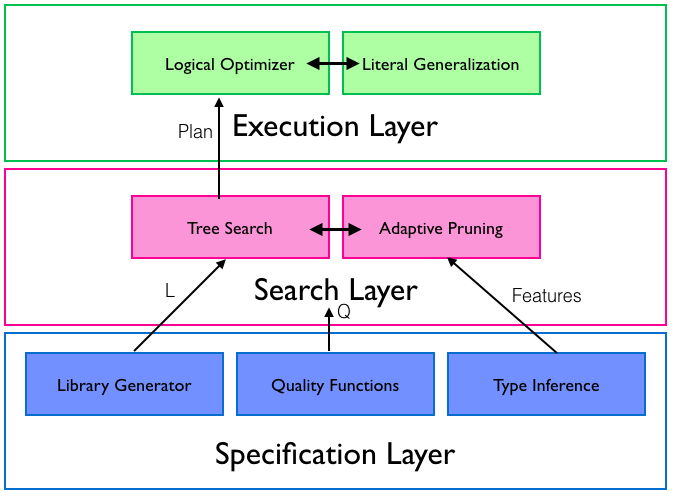
\includegraphics[width=\columnwidth]{figures/alphacleanarch.png}
 \caption{ \sys is given a specification of quality (e.g., integrity constraints or a statistical model the data must conform to) and a language  of  allowed  data  transformations,  and  it  searches  to find a sequence of transformations that maximizes the quality metric. }
\end{figure}


\subsection{System Architecture}

\textbf{TODO}

\begin{enumerate}
    \item Synthesis
    \item Generalization
    \item Optimization
\end{enumerate}





